\documentclass[12pt]{article}
\usepackage[dvips]{graphics}
\usepackage[english]{babel}
\usepackage{doublespace}
\usepackage{epsf}
\usepackage{fancybox}
\usepackage{fancyheadings}
\usepackage{float}
\usepackage{graphicx}
\usepackage{here}
\usepackage{isolatin1}
\usepackage{palatino}
\usepackage{picinpar}
\usepackage{psfig}
\usepackage{rotate}
\usepackage{subfigure}
\usepackage{sverb}
\usepackage{t1enc}
\usepackage{wrapfig}


\setlength{\topmargin}{0cm}
\setlength{\headheight}{1cm}
\setlength{\textheight}{23cm}
\setlength{\textwidth}{16cm}
\setlength{\oddsidemargin}{0cm}
\setlength{\evensidemargin}{0cm}
\setlength{\columnsep}{0.125in}
\setlength{\columnseprule}{0.5pt}
\setlength{\footskip}{1cm}
\setstretch{1.2}


%--------------------------------- styles
%--------------------------------
%
% Setting the width of the verbatim parts according to 80 tt chars
% Since it is tt, any char is fine
%
\newlength{\verbatimbox}
\settowidth{\verbatimbox}{\scriptsize\tt
xxxxxxxxxxxxxxxxxxxxxxxxxxxxxxxxxxxxxxxxxxxxxxxxxxxxxxxxxxxxxxxxxxxxxxxxxxxxxxxx
}

\newenvironment{sourcelisting}
  {\VerbatimEnvironment\par\noindent\scriptsize
   \begin{Sbox}\begin{minipage}{\verbatimbox}\begin{Verbatim}}%
  {\end{Verbatim}\end{minipage}\end{Sbox}

\setlength{\fboxsep}{3mm}\center\shadowbox{\TheSbox}\normalsize\par\noindent}

\newenvironment{commandline}
  {\VerbatimEnvironment\par\vspace*{2mm}\noindent\footnotesize
   \begin{Sbox}\begin{minipage}{.979\textwidth}\begin{Verbatim}}%
  {\end{Verbatim}\end{minipage}\end{Sbox}\setlength{\shadowsize}{2pt}%
  \shadowbox{\TheSbox}\normalsize\par\noindent}

%--------------------------------- page style --------------------------------
\pagestyle{fancy} \rhead{Place and route}
\lhead{PART 3} \rfoot{\thepage} \lfoot{ALLIANCE TUTORIAL} \cfoot{}
\setlength{\footrulewidth}{0.6pt}
%
%\begin{figure}[H]\centering
% \includegraphics[width=8cm,height=8cm]{.eps}
% \caption{}
% \label{Fig:}
%\end{figure}
%---------------------------------- document ---------------------------------
\begin{document}

\title{
               {\Huge ALLIANCE TUTORIAL \\}
    {\large
               Pierre \& Marie Curie University \\
                    year 2001 - 2002\\
    }
    \vspace{1cm}
    {\huge
                      PART 3\\
    		place and route
    }
}
\date{}
\author{
              Frederic AK\hspace{2cm} Kai-shing LAM
}

\maketitle
\begin{figure}[H]\centering
  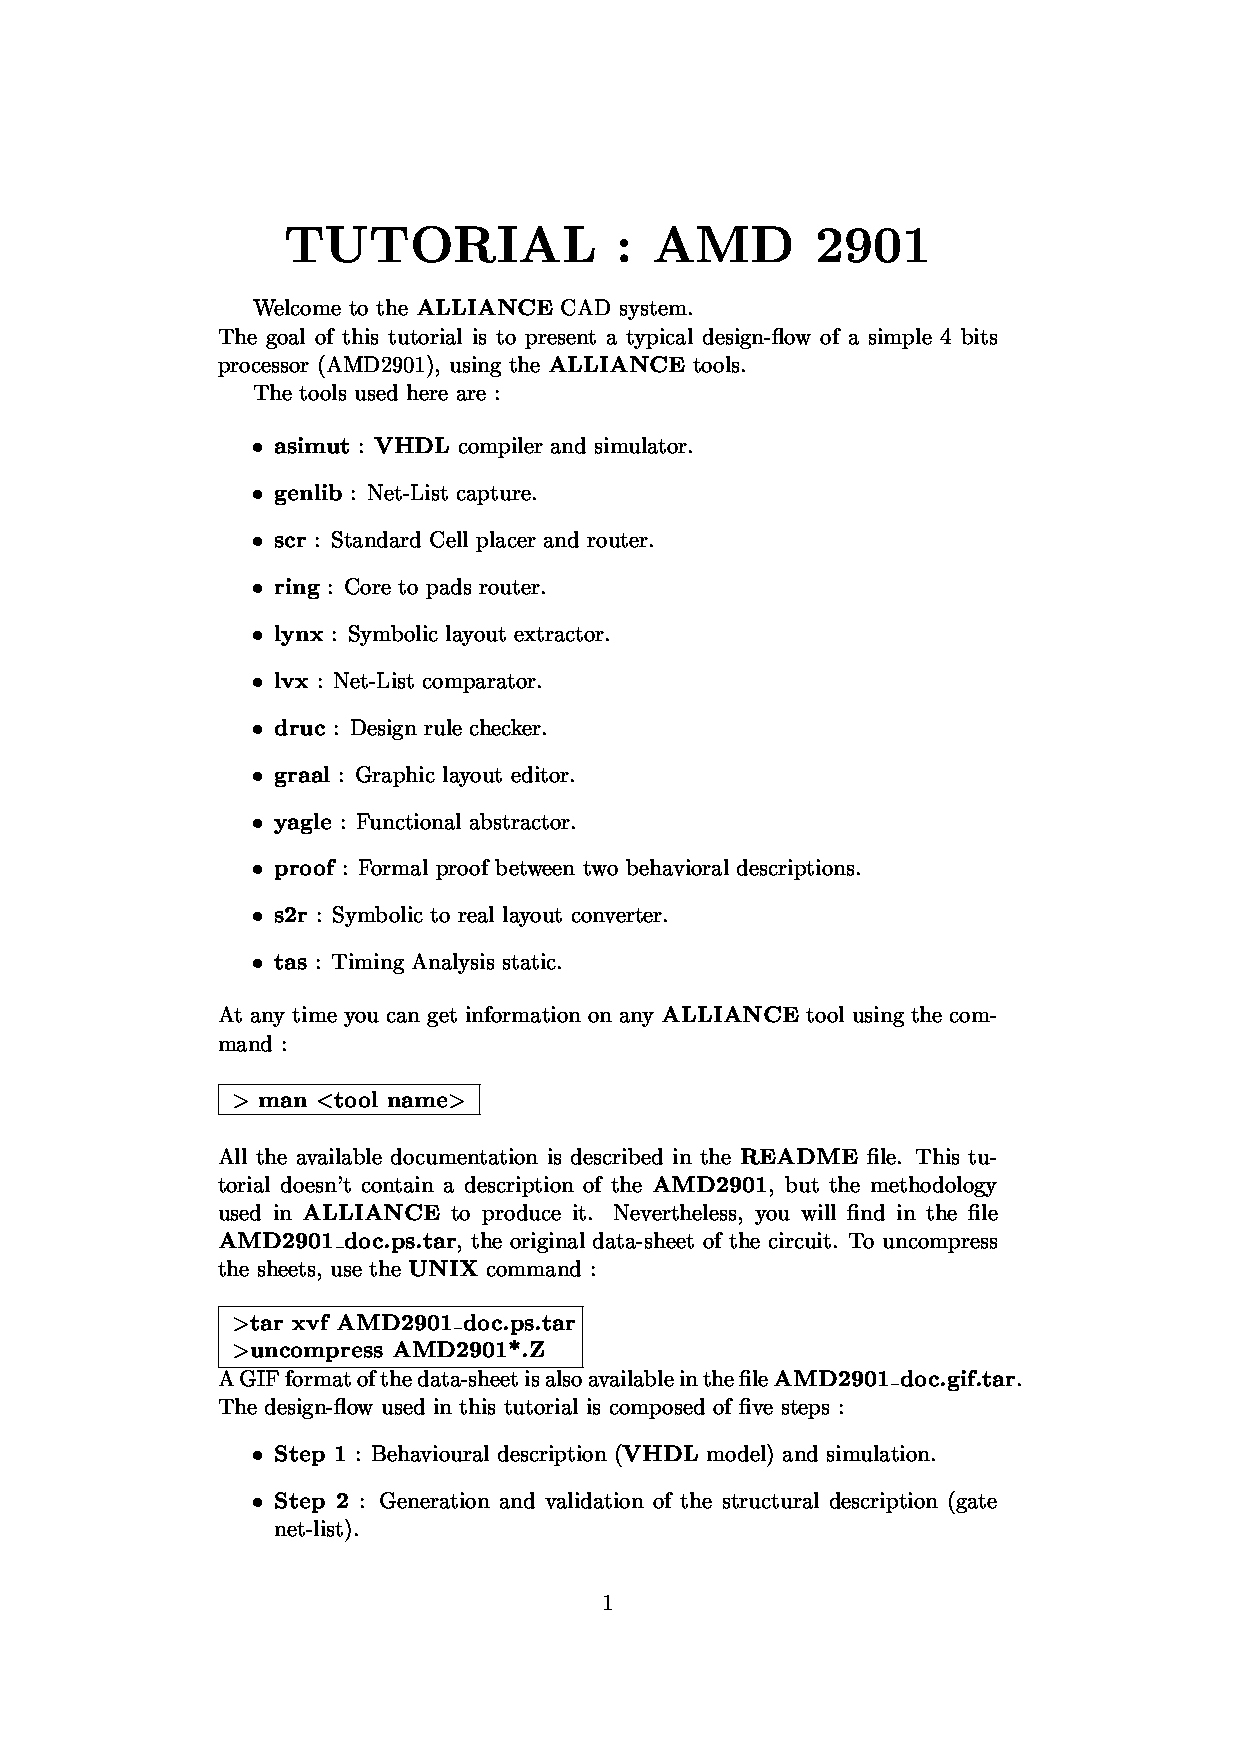
\includegraphics[height=10cm]{amd2901.epsi}
\end{figure}

\thispagestyle{empty}
\def\myfbox#1{\vspace*{3mm}\fbox{#1}\vspace{3mm}}
\newpage
{\bf Contents}\\
\\
{1} {\bf Introduction}
\\
{2 }{\bf Inversor and buffer drawing under GRAAL}

{2.1} Introduction

\hspace{0.5cm} {2.1.1} Technological environment

\hspace{0.5cm} {2.1.2} GRAAL

\hspace{0.5cm} {2.1.3} COUGAR

\hspace{0.5cm} {2.1.4} YAGLE

\hspace{0.5cm} {2.1.5} PROOF

{2.2} inversor Diagram

{2.3} Buffer diagram 

{2.4} sxlib gauge

{2.5} steps to follow

\hspace{0.5cm}  {2.5.1} Create an inversor

\hspace{0.5cm}  {2.5.2} Create a buffer
\\
{3} {\bf Place and Route}

{3.1} Amd2901 architecture

{3.2} Tools used

{3.3} Technological environment

{3.4} Beware of naming the files

{3.5} Data-path predefined placement

{3.6} heart Placement

{3.7} Route the heart

{3.8} pads placement
\\
{4} {\bf Annexes} 
 
\newpage
       {\huge
        PART 3 : }
        \vspace{1cm}
        {\huge
        Place and route
        }
 
All the files used in this part are located under \\
\texttt{/tutorial/place\_and\_route/src} directory.\\
This directory contents three subdirectories and one Makefile :

\begin{itemize}\itemsep=-.8ex

\item   Makefile
\item   inversor
    \begin{itemize}\itemsep=-.8ex
    \item   Makefile
    \item   inversor.vbe : behavioral description 
    \item   inv\_x1.ap : inversor cell under GRAAL
    \end{itemize}
\item   buffer
    \begin{itemize}\itemsep=-.8ex
    \item   Makefile
    \item   buffer.vbe : behavioral description
    \item   buf\_x2.ap : buffer cell under GRAAL
    \end{itemize}
\item  amd2901 
    \begin{itemize}\itemsep=-.8ex
    \item   Makefile
    \item   amd2901\_ctl.vbe : behavioral description of control
    part
    \item   amd2901\_dpt.vbe : behavioral description of data-path
    \item   amd2901\_ctl.c : file .c of control part
    \item   amd2901\_dpt.c : file .c of data-path
    \item   amd2901\_core.c : file .c of heart
    \item   amd2901\_chip.c : file .c of the circuit with their
    pads
    \item   pattern.pat : tests file
    \end{itemize}
\end{itemize}


\newpage

\section{Introduction}
%---------------------
 The goal of this tutorial is to present some ALLIANCE tools :
\begin{itemize}\itemsep=-.4ex
\item   {\bf GRAAL} Graphic layout editor ;
\item   {\bf DRUC} Design rule checker ;
\item   {\bf COUGAR} Symbolic layout extractor ;
\item   {\bf PROOF} Formal proof between two behavioral descriptions ;
\item   {\bf OCP, OCR, RING} place and route tools .
\end{itemize}

The beginning of this tutorial will relate to the drawing under {
\bf GRAAL } of a inversor cell and a buffer.
The predefined cells concepts, model and
hierarchy will be introduced .\\
Then this tutorial contain the methodology used in Alliance to produce
the amd2901 physical layout that you conceived in Alliance Tutorial 
PART 2 "Synthesis" (All the documents used will be provided to you).
 
\newpage
%%%%%%%%%%%%%%%%%%%%%%%%%%%%%%%%%%%%%%%%%%%%%%%%%%%%%%%%%%%%%

\section{Inversor and buffer drawing under GRAAL}
%-----------------------------------------------

\subsection{Introduction}
%------------------------
    The library can be enriched by new cells with {\bf GRAAL} editor .\\
{ \bf GRAAL } is an editor of \/{\underline{symbolic }} {\it
layout} integrating the drawing rules checker {\bf DRUC}. The
first part here aims to draw a inversor cell inv\_x1 in the shape
of a predefined cell sxlib  by complying with the provided
drawing rules.

\subsubsection{Technological environment}
%--------------------
Some tools of Alliance use a particular technological
environment. It is indicated by the environment variable {\bf
RDS\_TECHNO\_NAME} which must be positioned with
{\bf/asim/alliance/etc/cmos\_12.rds}

\subsubsection{GRAAL}
%--------------------
    The {\it layout } editor \/handles six different objects types which we can create
    with the menu { \bf CREATE }:
\begin{itemize}\itemsep=-.4ex
\item   The ''instance'' (physical cells importation)
\item   The abutment boxes which define the cell limits 
\item   Segments: DiffN, DiffP, Poly, Alu1, Alu2... CAluX is used to indicate
        a possible portion for the connectors.
\item   VIAs or contacts: ContDiffN, ContDiffP, ContPoly and
    ViaMetal1/Metal2.
\item   Big VIAs
\item   Transistors: NMOS or PMOS
\end{itemize}

{\bf GRAAL} uses the environment variable {\bf
GRAAL\_TECHNO\_NAME}. It must be positioned with
{\bf/asim/alliance/etc/cmos\_12.graal}.

Steps to follow to create a sxlib cell by respecting the sxlib gauge :
( cf 2.4 Sxlib gauge ) 
\begin{itemize}\itemsep=-.4ex
\item	place the supply Vdd and Vss using the menu CREATE->Segment
\item	place the VIAs using the menu CREATE->VIA
\item 	place the transistors PMOS and NMOS using the menu CREATE->Transistor
\item	place the NWell body using the menu CREATE->Segment
\item 	place the input/output connectors using the menu CREATE->VIA
\item	link the transistor P and the transistor N with the Poly segment using the menu CREATE->Segment
\item	supply each transistor by linking them with Ndiff and Pdiff segments and VIAs contacts
\item 	define the cell limit with an abutment box using the menu CREATE->Abutment Box
\end{itemize} 

\subsubsection{COUGAR}
%--------------------
The tool { \bf COUGAR } is able to extract the { \it netlist } from
a circuit to the format { \bf vst } starting from a description
with the format { \bf ap }. To extract on the level transistor,
the command to be used is:

\begin{commandline}
 > cougar -t file1 file2 
\end{commandline}

{ \bf COUGAR } uses the environment variables { \bf MBK\_IN\_PH }
and { \bf MBK\_OUT\_LO } according to the input and output formats.
For example to generate a netlist with the format { \bf .al } 
starting from a description { \bf .ap } it is necessary to write: \\

\begin{commandline}
 > MBK_IN_PH = ap 
 > export MBK_IN_PH 
 > MBK_OUT_LO = al 
 > export MBK_OUT_LO
\end{commandline}

\begin{commandline}
 > cougar -t circuit circuit  
\end{commandline}

\subsubsection{YAGLE}
%--------------------
The tool { \bf YAGLE } is able to extract the behavioral
VHDL description of a circuit to the format { \bf .vbe } starting
from a { \it netlist } \/with the format { \bf .al } { \it if this
one is on the transistor level }.
The command to be used is: \\

\begin{commandline}
 > MBK_IN_LO = al 
 > export MBK_IN_LO 
 > YAGLE_BEH_FORMAT = vbe 
 > export YAGLE_BEH_FORMAT
\end{commandline}

\begin{commandline} 
 > yagle file1 file2
\end{commandline} 

Above all, you must use the command:
\begin{commandline}
 > source /users/soft5/newlabo/AvtTools/etc/avt_env.csh 
\end{commandline}
which allows to set up the environment necessary to use { \bf YAGLE }.\\
Documentations for this tool are in :
{\bf/users/soft5/newlabo/AvtTools/doc}

But the tool { \bf YAGLE } is not part of Alliance anymore. If you want
to use it, you have to get the licence from Avertec. 

\subsubsection{PROOF}
%--------------------
When we want to prove the equivalence between two behavioral
descriptions of the same circuit with N inputs, we can simulate
by asimut $2^n$ vectors for two descriptions and compare them.
This solution quickly becomes expensive in CPU time and it is 
better to use formal proof tool which carries out the
"mathematical" comparison of the two Boolean networks. { \bf PROOF
} carries out this operation between descriptions file1.vbe and
file2.vbe by the command:

\begin{commandline}
 > proof file1 file2 
\end{commandline}

\subsection{inversor Diagram}
%---------------------------------

The theoretical inversor diagram is presented at the following
figure:

\begin{figure}[H]\centering
  \includegraphics[width=6cm]{inv_x1.eps}
  \caption{transistors diagram of a C-MOS inversor}
  \label{Fig:inv_x1}
\end{figure}

\subsection{Buffer diagram }
%---------------------------------

The theoretical buffer diagram is presented at the following
figure:

\begin{figure}[H]\centering
  \includegraphics[width=8cm]{buff_x1.eps}
  \caption{transistors diagram of a C-mos buffer}
  \label{Fig:buff_x1}
\end{figure}

It uses two inversors according to the hierarchy:

\begin{figure}[H]\centering
  \includegraphics[width=8cm]{hierarchie.eps}
  \caption{C-mos buffer hierarchy}
  \label{Fig:hier_x1}
`\end{figure}

\subsection{sxlib gauge}
%---------------------------------

\begin{itemize}\itemsep=-.4ex
\item The sxlib cells have whole 50 lambdas height and a multiple of 5 lambdas width.
\item The supply Vdd and Vss are carried out in Calu1; they have 6 lambdas width and are 
horizontally placed in top and bottom of the cell.
\item The transistors P are placed close to the Vdd while transistors N are placed close
        to the Vss.
\item Box N must have 24 lambdas height .
\item The special segments CAluX (CAlu1, Calu2, CAlu3...) form the cell interface (PORT\_MAP) 
and play the role of ''flat'' connectors. They must {\underline{obligatorily}}
be placed on a 5x5 grid and can be anywhere in the cell.
\item The special segments TAlux (TAlu1, TAlu2...) are used to indicate the obstacles for the
        router. When you want to protect AluX segment, it is necessary to cover them
        or surround them by corresponding TAlux (same layer). TAluX are placed on a grid
        with 5 lambdas steps (figure \ref{Fig:gabarit2}).
\item The minimal width of CAlu1 is 2 lambda, plus 1 lambda for the extension (figure \ref{Fig:gabarit3}).
\item The boxes N and P must be polarized. { \bf It should be respectively connected to Vdd and Vss }.
\end{itemize}

You will find a summary of these constraints on the diagram 
\ref{Fig:gabarit}:

\begin{figure}[H]\centering
  \includegraphics[scale=0.8]{gabarit_sx.eps}
  \caption{a cell model of the sxlib library }
  \label{Fig:gabarit}
\end{figure}

\begin{figure}[H]\centering
  \includegraphics[scale=0.8]{gabarit2_sx.eps}
  \caption{Use the layer TAluX like protection}
  \label{Fig:gabarit2}
\end{figure}

\begin{figure}[H]\centering
  \includegraphics[scale=0.8]{gabarit3_sx.eps}
  \caption{Low size of CAlu1}
  \label{Fig:gabarit3}
\end{figure}

\subsection{steps to follow}
%---------------------------------

\subsubsection{Create an inversor}
%--------------------

\begin{itemize}\itemsep=-.4ex
\item   describe the cell inversor behavior in a file { \bf .vbe } .
\item   draw the inversor "stick-diagram" inv\_x1 whose transistors diagram
        is represented on the figure \ref{Fig:inv_x1}.

\begin{figure}[H]\centering
  \includegraphics[width=8cm]{stick.eps}
  \caption{stick diagram}
  \label{Fig:stick}
\end{figure}

\item   draw the cell under {\bf GRAAL} by respecting the
        gauge specified on the figure \ref{Fig:gabarit}.
\item   validate the symbolic drawing rules by launching {\bf DRUC} under {\bf GRAAL}.
\item   extract the { \it netlist } \/from the inversor to the format {\bf al} with {\bf COUGAR}.
\item   extract the behavioral VHDL with { \bf YAGLE }
\item   carry out the formal proof between the file { \bf .vbe } extracts by { \bf YAGLE }
        and the file { \bf .vbe } from the initial specification.
\end{itemize}

\subsubsection{Create a buffer}
%--------------------

The buffer is produced under { \bf GRAAL } starting from the
instanciated of two inversors. The hierarchy thus created is
represented on the figure \ref{Fig:hier_x1}. The transistors
diagram is represented on the figure \ref{Fig:buff_x1}.

\begin{itemize}\itemsep=-.4ex
\item   describe the cell buffer behavior in a file { \bf .vbe }.
\item   draw the cell under {\bf GRAAL} by respecting the
        gauge specified on the figure \ref{Fig:gabarit}.
        You will use for that the instanciated function of { \bf GRAAL }.
        The cell with instanciate is of course the inversor, which you will connect (will routing) manually.
\item   validate the symbolic drawing rules by launching {\bf DRUC} under {\bf GRAAL}.
\item   extract the { \it netlist } \/from the buffer to the format {\bf al} with {\bf COUGAR}.
\item   extract the behavioral VHDL with { \bf YAGLE }
\item   carry out the formal proof between the file { \bf .vbe } extracts by { \bf YAGLE }
        and the file { \bf .vbe } from the initial specification.
\end{itemize}

Do not forget that the { \it mans } exist...
We provide you the cells behaviour description inversor.vbe and buffer.vbe;
and the cells inversor and buffer draws under { \bf GRAAL }.

%%%%%%%%%%%%%%%%%%%%%%%%%%%%%%%%%%%%%%%%%%%%%%%%%%%%%%%%%%%%%

\section{Place and Route}
%-------------------

\subsection{Amd2901 architecture}
%---------------------------------

Am2901 breaks up into 2 blocks: the part controls which gathers
the logical `` glu '' and the operative part (data-path).

\begin{figure}[H]\centering
  \includegraphics[scale=0.8]{bloc.eps}
  \caption{Amd decomposition in functional units}
  \label{Fig:decomposition}
\end{figure}


\begin{itemize}\itemsep=-.4ex
\item The data-path contains the regular parts of Amd2901, the registers
     and the arithmetic logic unit.
\item The control part contains irregular logic, 
    the instructions decoding and the `` flags '' calculation.
\end{itemize}

Hierarchical description used is as follows:

\begin{figure}[H]\centering
  \includegraphics[scale=0.8]{hier.eps}
  \caption{Hierarchy used}
  \label{Fig:hierarchie}
\end{figure}

\subsection{Tools used}
%---------------------------------

You will use place and route tools { \bf ocp } and {\bf ocr },
thus all tools for checking seen in the first part of this Tutorial .\\
{\bf ocp} is the placer, {\bf ocr} allows routing over the cell.
The data-path and the control part will be placed and routed together and not separately. \\
You will use also {\bf lvx}, the netlists comparator. When the
system is too complex it is difficult to use {\bf proof}, the
formal comparator (calculations too long). A netlists comparison 
then is used. Test the two methods ({\bf proof} and {\bf
lvx}).

\subsection{Technological environment}
%---------------------------------

\begin{sourcelisting}
 > VH_MAXERR = 10
 > export VH_MAXERR
 > MBK_WORK_LIB = .
 > export MBK_WORK_LIB
 > MBK_CATA_LIB = $ALLIANCE_TOP/cells/sxlib
 > export MBK_CATA_LIB
 > MBK_CATA_LIB = $MBK_CATA_LIB:$ALLIANCE_TOP/cells/dp_sxlib
 > export MBK_CATA_LIB
 > MBK_CATA_LIB = $MBK_CATA_LIB:$ALLIANCE_TOP/cells/padlib
 > export MBK_CATA_LIB
 > MBK_CATA_LIB $MBK_CATA_LIB:.
 > export MBK_CATA_LIB
 > MBK_CATAL_NAME = CATAL
 > export MBK_CATAL_NAME
 > MBK_IN_LO = vst
 > export MBK_IN_LO
 > MBK_OUT_LO = vst
 > export MBK_OUT_LO
 > MBK_IN_PH = ap
 > export MBK_IN_PH
 > MBK_OUT_PH = ap
 > export MBK_OUT_PH
\end{sourcelisting}

\subsection{Beware of naming the files}
%---------------------------------

Generally, the files describing a logical netlist must be the same
name as the corresponding file describing the physical netlist.
the file amd2901\_dpt.vst (LOFIG) must correspond to the file
amd2901\_dpt.ap (PHFIG). The same applies to the file
amd2901\_core. Check well that you do not overwrite a file!

\subsection{Data-path predefined placement}
%---------------------------------

For the moment, your file amd2901\_dpt.c contains only one logical
description of the netlist.
eg you have a file C which contains the lines: \\

\noindent GENLIB\_DEF\_LOFIG()\\
\noindent ...\\
\noindent GENLIB\_SAVE\_LOFIG()\\

That enables you to generate a description structural in file{ \bf
VST }. But at the same time, { \bf genlib } generated physical
descriptions of each column in files { \bf AP }.
It is about placing these columns explicitly. \\
Take again the file amd2901\_dpt.c and include the lines :\\

\noindent GENLIB\_DEF\_PHFIG()\\
\noindent ...\\
\noindent GENLIB\_SAVE\_PHFIG()\\

The suspension points are to be supplemented, they represent your
operators placement. You have for, that {\bf
GENLIB} functions : 

\begin{itemize}\itemsep=-.4ex
\item GENLIB\_PLACE()
\item GENLIB\_PLACE\_RIGHT()
\item GENLIB\_PLACE\_TOP()
\item GENLIB\_PLACE\_LEFT()
\item GENLIB\_PLACE\_BOTTOM()
\item GENLIB\_PLACE\_ON()
\item GENLIB\_DEF\_AB()
\item ...
\end{itemize}

Use {\bf GENLIB} manual. The placement of the  data
path columns should not be made randomly. The routing depends on it.\\

Use genlib to generate all:

\begin{commandline}
 >genlib  amd2901_dpt 
\end{commandline}

The figure \ref{Fig:preplacement} summarizes the followed process:

\begin{figure}[H]\centering
  \includegraphics[scale=0.8]{preplacement.eps}
  \caption{predefined placement}
  \label{Fig:preplacement}
\end{figure}

\begin{figure}[H]\centering
  \includegraphics[scale=0.8]{colonnes.eps}
  \caption{predefined Columns before placement of the part controls }
  \label{Fig:colonnes}
\end{figure}

Do not forget to include a abutment box!

\subsection{heart Placement}
%---------------------------------

Same manner, take again the file amd2901\_core.c and place data
path explicitly. You should not place the part controls. This one
exists only in the form of a structural description. It is the
placer { \bf ocp } which will undertake some (during the placement
of the heart { \bf ocp } detects which are the cells not placed
and supplements the placement). You should nevertheless envisage
space for the cells placement { \bf to the top } of the
data-path.

Include the lines:\\

\noindent GENLIB\_DEF\_PHFIG()\\
\noindent ...\\
\noindent GENLIB\_SAVE\_PHFIG()\\

The suspension points represent the placement of data-path. Space
necessary to the placer to place the cells of the control part
will be determined by successive approximations. You will have to
adjust dimensions of the heart abutment box 
(GENLIB\_DEF\_AB()).
Use the command:

\begin{commandline}
 > genlib  amd2901_core 
\end{commandline}

and
\begin{commandline}
 > ocp -partial amd2901_core -ioc amd2901_core amd2901_core amd2901_core_p 
\end{commandline}

The option {\bf -- partial} indicates that you transmit a partial
placement of the data-path. The option { \bf -- ioc }
request the loading of a file giving the placement of the
connectors. This file, amd2901\_core.ioc is provided to you
(Modify it according to your predefined placement. The connectors
must be in north and the south). The third argument is the netlist
heart, the fourth is the file { \bf AP } result.

The figure \ref{Fig:placement} summarize the followed process:

\begin{figure}[H]\centering
  \includegraphics[scale=0.6]{placement.eps}
  \caption{Placement}
  \label{Fig:placement}
\end{figure}

\subsection{Route the heart}
%---------------------------------

Routing the heart by using { \bf ocr } in the following way:

\begin{commandline}
 > ocr  -P amd2901_core_p -L amd2901_core -O amd2901_core -l 3 -v -i 30
\end{commandline}

%The option { \bf -- place } indicates that you transmit a placement, that of the heart.
%The third argument is the netlist heart, the fourth is the file { \bf AP } result. \\

%{\bf NOTA}:
%\begin{itemize}\itemsep=-.4ex
%\item   Variable MBK\_CATA\_LIB should contain only once the access paths to the libraries.
%\item   The file of error generated by { \bf ocr } is {\bf .log}.
%{ \bf THIS FILE MUST BE IMPERATIVELY CONSULTS } before beginning
%the following stages. Indeed, it is thanks to this file that the
%router informs you if it made a success of with routing all the
%signals or not...
%\end{itemize}

\subsection{pads placement}
%---------------------------------

The heart is now completed. The pads still should
be added allowing the connection of the inputs/outputs to the case. \\
The tool {\bf ring} allows to instanciate the pads it has need
for signals list describing the relations between the heart
and the pads, as well as a file { \bf .rin } specifying the
geometrical provision of the crown of pads. \\

This file uses syntax:
\begin{sourcelisting}
 > east ( pi1 pi0 )
 > west ( pck pi4 )
 > north ( pvdd pvss )
 > south ( pvdde pvsse )
\end{sourcelisting}

Where pi1, pi0... are the names of the pads ''instances''.
Name it `` amd2902\_chip.rin '' and apply the command \\

\begin{commandline}
 > ring amd2901_chip amd2901_chip 
\end{commandline}

We will validate the work of {\bf ring} with the tools { \bf druc
}, { \bf lynx } and { \bf lvx }.\\

Validate the drawing rules:
\begin{commandline}
 > druc amd2901_chip
\end{commandline}
Extract the symbolic layout and flattened it:
\begin{commandline}
 > MBK_OUT_LO = al
 > export MBK_OUT_LO
\end{commandline}

\begin{commandline}
 > cougar -f amd2901_chip
\end{commandline}
Compare two netlists : 
\begin{commandline}
 > lvx vst al amd2901_chip amd2901_chip -f
\end{commandline}

\begin{commandline}
 > MBK_OUT_LO = vst
 > export MBK_OUT_LO
\end{commandline}

simulated the file extracts with { \bf asimut }.
Pay attention to the file { \bf CATAL }!\\
To know the number of transistors, we carry out an extraction of
the circuit on the level transistor: \\

\begin{commandline}
> cougar -t amd2901_chip amd2901_chip 
\end{commandline}
\\

If you want to see the amd2901 control part :
\begin{commandline}
> make view_ctl_logic
\end{commandline}
 
If you want to see the data-path physical layout:
\begin{commandline}
> make view_dpt_physic
\end{commandline}

note: you can see in red the critical path.

If you want to see the chip physical layout:
\begin{commandline}
> make view_chip_physic
\end{commandline}

If you want to see the different propagation times:
\begin{commandline}
> make view_chip_simulation
\end{commandline}
     
%%%%%%%%%%%%%%%%%%%%%%%%%%%%%%%%%%%%%%%%%%%%%%%%%%%%%%%%%%%%%

%\newpage
%\section{Conclusion}
%-------------------
%    This Tutorial enabled you to pass by the majority of the stages necessary to
%    the design and the validation of a circuit carried out in precaracterized cells. \\


\newpage

\section{Annexes}
%-------------------

\begin{figure}[H]\centering
  \includegraphics[scale=0.8]{dpt-all-1.eps}
  \caption{data-path general view }
  \label{Fig:dpt}
\end{figure}

%%%%%%%%%%%%%%%%%%%%%%%%%%%%%%%%%%%%%%%%%%%%%%%%%%%%%%%%%%%%%
%%%%%\cleardoublepage
\newpage

%\vfill

\newpage

%\vfill

\end{document}
